\documentclass{fizraport}
\authorA{Krzysztof Stasiowski}
\authorB{Joanna Binek}
\team{2}{2a}{1}

\topic{Wahadło fizyczne}{1}{
Opis ruchu drgającego, a~w~szczególności drgań wahadła fizycznego. Wyznaczenie momentów bezwładności brył sztywnych.
}
\carryOutDate{10.10.2018 r.}
\ftHandInDate{17.10.2018 r.}
\begin{document}

\maketitle
\vfill

\section{Układ pomiarowy}

\begin{enumerate}
    \item Statyw, na którym zawiesza się badaną bryłę
    \item Badane bryły: pręt, pierścień
    \item Metalowy przymiar milimetrowy
    \item Suwmiarka
    \item Waga elektroniczna
    \item Sekundomierz
\end{enumerate}

\begin{figure}[htbp]
 \centering
 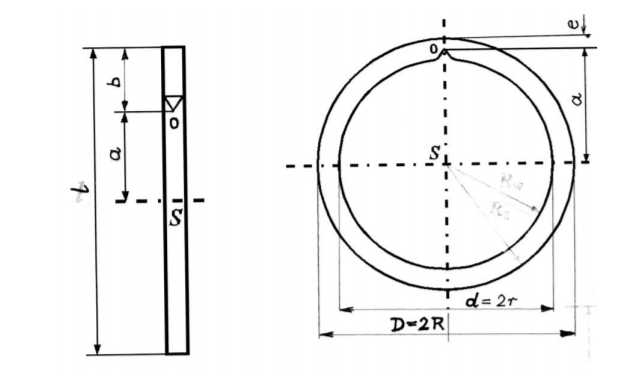
\includegraphics[width=0.6\textwidth,keepaspectratio=true]{rysunek1.png}
 \label{fig:pret}
   \caption{Pręt i pierścień używane w ćwiczeniu.}
\end{figure}
\vfill

%będe tu testował parę rzeczy - nie przeszkadzaj sobie, ja zabiorę się za to raczej dopiero w weekend
%\addplot[rlc]{caption}{id}{plot}{width}
%\addplot{Pręt i pierścień używane w ćwiczeniu.}{w1}{rysunek1.png}{0.7\textwidth}
%\addplot[c]{Pręt i pierścień używane w ćwiczeniu.}{w1}{rysunek1.png}{0.7\textwidth}
%\addplot[l]{Pręt i pierścień używane w ćwiczeniu.}{w1}{rysunek1.png}{0.7\textwidth}
%\addplot[p]{Pręt i pierścień używane w ćwiczeniu.}{w1}{rysunek1.png}{0.7\textwidth}

%\uncertain{1.23}{13} normalna
%\uncertain[e]{1.23}{26} rozszeżona
%$\uncertain[e]{1.23}{13}$
%$\uncertain{1.23}{26}$
%end test area
\pagebreak
\section{Opis doświadczenia} 
Na początku wykonywania doświadczenia zmierzyliśmy masę pręta i~pierścienia przy użyciu wagi w laboratorium o~dokładności~1g.

Następnie wyznaczyliśmy rozmiary pręta i~pierścienia zaznaczone na \figref{fig:pret} przy pomocy linijki o~podziałce~1mm. Jeśli któraś długość była relatywnie mała to do pomiaru użyliśmy suwmiarki o~dokładności~0.05mm. W przypadku długości $a$ zastosowaliśmy niepewność 5.05mm z powodu konieczności wyznaczenia środka masy $S$ dla obu brył.

Dodatkowo niektóre z wymiarów pręta (promień zewnętrzny, promień wewnętrzny) wyliczyliśmy samodzielnie przy pomocy obliczeń arytmetycznych na~podstawie pobranych pomiarów.

Po zakończeniu pomiarów umieściliśmy pręt na~statywie, a~następnie wprowadziliśmy go w ruch wychylając go o~niewielki kąt i~puszczając. Za pomocą stopera o~dokładności~0.01s zmierzyliśmy czas 15~drgań pręta. Do niepewności pomiaru stopera należy dodać czas reakcji osoby wykonującej pomiar, który został ustalony na~0.1s. Czynności powtórzyliśmy dziesięciokrotnie.

Po zakończeniu serii pomiarów dla pręta, wykonaliśmy ją dla pierścienia według tego samego schematu.
Zebrane dane przedstawiliśmy w~tabelach~\tabref{tab:pomiarWym}~i~\tabref{tab:pomiarOkres}
\begin{table}[h]
\caption{Pomiary masy i długości}
\centering

\begin{tabular}{|l|l|l|}

\hline
\multicolumn{3}{|c|}{Pręt}      \\ \hline
         & wartość & niepewność \\ \hline
$m$ [g]  & 651     & 1          \\ \hline
$l$ [mm] & 750     & 1          \\ \hline
$b$ [mm] & 96      & 0.05       \\ \hline
$a$ [mm] & 380     & 5.05       \\ \hline 
\end{tabular}
\quad
\begin{tabular}{|l|l|l|}
\hline
\multicolumn{3}{|c|}{Pierścień} \\ \hline
          & wartość & niepewność\\ \hline
$m$ [g]  & 1331    & 1          \\ \hline 
$Dw$[mm] & 251     & 1          \\ \hline
$Dz$[mm] & 279     & 1          \\ \hline
$Rw$[mm] & 125.5   & 0.5        \\ \hline 
$Rz$[mm] & 139.5   & 0.5        \\ \hline
$e$ [mm] & 9       & 0.05       \\ \hline
$a$ [mm] & 123.3   & 5.05       \\ \hline 
\end{tabular}
 \label{tab:pomiarWym}
\end{table}

\begin{table}[th]
\caption{Pomiary okresu drgań}
\newlength{\colW}
\setlength{\colW}{1.45cm}
\centering
\begin{tabular}{|r|c|c|c|}
\hline
\multicolumn{4}{|c|}{Pręt} \\ \hline
\multirow[t]{3}{0.5\colW}{\centering\textbf{Lp.}}&
\multirow[t]{3}{\colW}{\centering \textbf{Liczba okresów $k$}}&
\multirow[t]{3}{1.5\colW}{\centering\textbf{ Czas $t[s]$ dla $k$ okresów}}&
\multirow[t]{3}{\colW}{\centering\textbf{Okres $T_i[s]$}}\\
&&&\\&&&\\\hline
1 & 15 & 19.79 & 1.32 \\ \hline
2& 15 & 19.79 & 1.32 \\ \hline
3& 15 & 19.97 & 1.33 \\ \hline
4& 15 & 20.00 & 1.33 \\ \hline
5 & 15 & 20.06 & 1.34 \\ \hline
6& 15 & 19.88 & 1.33 \\ \hline
7& 15 & 19.91 & 1.33 \\ \hline
8& 15 & 19.94 & 1.34 \\ \hline
9& 15 & 19.72 & 1.31 \\ \hline
10& 15 & 19.94 & 1.34 \\ \hline


\multicolumn{4}{|l|}{Wartość średnia okresu $T_I$:   1.3267 } \\ \hline
\multicolumn{4}{|l|}{Niepewność $u(T_I)$:  0.0022 } \\ \hline
\end{tabular}
\quad
\begin{tabular}{|r|c|c|c|}
\hline
\multicolumn{4}{|c|}{Pierścień} \\ \hline
\multirow[t]{3}{0.5\colW}{\centering\textbf{Lp.}}&
\multirow[t]{3}{\colW}{\centering \textbf{Liczba okresów $k$}}&
\multirow[t]{3}{1.5\colW}{\centering\textbf{ Czas $t[s]$ dla $k$ okresów}}&
\multirow[t]{3}{\colW}{\centering\textbf{Okres $T_i[s]$}}\\
&&&\\&&&\\\hline
1 & 15 & 15.38 & 1.025 \\ \hline
2& 15 & 15.47 & 1.031 \\ \hline
3& 15 & 15.35 & 1.023 \\ \hline
4& 15 & 15.47 & 1.031 \\ \hline
5 & 15 & 15.29 & 1.019 \\ \hline
6& 15 & 15.35 & 1.023 \\ \hline
7& 15 & 15.44 & 1.029 \\ \hline
8& 15 & 15.35 & 1.023 \\ \hline
9& 15 & 15.54 & 1.036 \\ \hline
10& 15 & 15.47 & 1.031 \\ \hline

\multicolumn{4}{|l|}{Wartość średnia okresu $T_o$:   1.0274} \\ \hline
\multicolumn{4}{|l|}{Niepewność $u(T_o)$:  0.0016 } \\ \hline
\end{tabular}
 \label{tab:pomiarOkres}
\end{table}

\pagebreak
\section{Opracowanie wyników:}
\subsection{Obliczenie momentu bezwładności $I_0$ względem rzeczywistej osi obrotu korzystając ze~wzoru na~okres
drgań}
Okres drgań $T$ w~ruchu harmonicznym przedstawia się wzorem:
\begin{equation*}
T = 2\pi\sqrt{\frac{I_0}{mga}}
\end{equation*}
co po przekształceniu daje wzór roboczy na~moment bezwładności~$I_0$
\begin{equation*}
I_0 = \frac{T^2mga}{4\pi^2}
\end{equation*}
\subsubsection{Moment bezwładności dla pręta}
\begin{equation*}
I_0 = \frac{T^2mga}{4\pi^2}=\frac{1.3267^2\cdot0.651\cdot9.81\cdot0.38}{4\pi ^2}=0,11~\left[kg\cdot m^2\right]
\end{equation*}
\subsubsection{Moment bezwładności dla pierścienia}
\begin{equation*}
I_0 = \frac{T^2mga}{4\pi^2}=\frac{1.0274^2\cdot1.331\cdot9.81\cdot0.1233}{4\pi ^2}=0.0431~\left[kg\cdot m^2\right]%0.04304821447573781
\end{equation*}

\subsection{Obliczenie momentu bezwładności $I_S$~względem osi przechodzącej
przez środek masy korzystając z~twierdzenia Steinera}
Do obliczenia momentu bezwładności $I_S$ wahadła fizycznego można posłużyć się również twierdzeniem Steinera, które ma postać:
\begin{equation*}
I_0 = I_s + ma^2
\end{equation*}
Chcąc obliczyć moment bezwładności~$I_S$~względem osi przechodzącej przez środek masy przekształcamy powyższe równanie do~postaci:
\begin{equation*}
I_s = I_0 - ma^2
\end{equation*}
\subsubsection{Obliczenia dla pręta:}
Po podstawieniu wcześniej wyliczonego doświadczalnie $I_0$ oraz masy pręta i~odległości $a$ otrzymujemy wynik:
\begin{equation*}
I_s = I_0 - ma^2 = 0.11 - 0.651\cdot0.38^2= 0.016~\left[kg\cdot m^2\right]
\end{equation*}
\subsubsection{Obliczenia dla pierścienia:}
Po podstawieniu wcześniej wyliczonego doświadczalnie $I_0$ oraz masy pierścienia i~odległości $a$ otrzymujemy wynik:
\begin{equation*}
I_s = I_0 - ma^2 = 0.043 - 1.331\cdot0.1233^2= 0.023~\left[kg\cdot m^2\right]%0.02281316788573781
\end{equation*}
\subsection{Niepewności złożone momentu bezwładności $I_0$ oraz $I_S$}
Niepewności złożone obliczamy dla momentu bezwładności pierścienia $u(I_0)$. % tu jakoś trzeba dodać więcej tekstu 
\begin{align*}
    \frac{u(I_0)}{I_0} &=\sqrt{
    \left( \frac{ \partial I_0 }{ \partial T} \frac{T}{I_0} \frac{u(T)}{T}\right)^2+
    \left( \frac{ \partial I_0 }{ \partial m} \frac{m}{I_0} \frac{u(m)}{m}\right)^2+
    \left( \frac{ \partial I_0 }{ \partial a} \frac{a}{I_0} \frac{u(a)}{a}\right)^2
    }\\
    \left( \frac{ \partial I_0 }{ \partial T} \frac{T}{I_0}\right) &=
    \left( \frac{2Tga}{4\pi^2}  \frac{1}{\frac{Tga}{4\pi^2}}\right) = 2\\
    \left( \frac{ \partial I_0 }{ \partial m} \frac{m}{I_0}\right) &=
    \left( \frac{T^2ga}{4\pi^2}  \frac{1}{\frac{T^2ga}{4\pi^2}}\right) = 1\\
    \left( \frac{ \partial I_0 }{ \partial a} \frac{a}{I_0}\right) &=
    \left( \frac{T^2gm}{4\pi^2}  \frac{1}{\frac{T^2gm}{4\pi^2}}\right) = 1\\
    \frac{u(I_0)}{I_0} &=\sqrt{
    \left( 2 \frac{u(T)}{T}\right)^2+
    \left( 1 \frac{u(m)}{m}\right)^2+
    \left( 1 \frac{u(a)}{a}\right)^2
    }=0.042\\ %0.0410917
    I_0&=\uncertain{0.0431}{18}\left[kg\cdot m^2\right]
\end{align*}
Następnie wykorzystujemy je do obliczenia $u(I_S)$
\begin{align*}
    \frac{u(I_0)}{I_0} &=\sqrt{
    \left( \frac{ \partial I_S }{ \partial I_0} \frac{I_0}{I_S} \frac{u(I_0)}{I_0}\right)^2+
    \left( \frac{ \partial I_S }{ \partial m} \frac{m}{I_S} \frac{u(m)}{m}\right)^2+
    \left( \frac{ \partial I_S }{ \partial a} \frac{a}{I_S} \frac{u(a)}{a}\right)^2
    }\\
    %
    \left( \frac{ \partial I_S }{ \partial I_0} \frac{I_0}{I_S}\right) &=
    \left( 1  \frac{I_0}{I_0-ma^2}\right) = 
    \left( \frac{1}{1-\frac{ma^2}{I_0}}\right)=-1.89\\%-1.888868
    %
    \left( \frac{ \partial I_S }{ \partial m} \frac{m}{I_S}\right) &=
    \left( a^2  \frac{1}{\frac{I_0}{m}-a^2} \right) = 
    \left(  \frac{1}{\frac{I_0}{ma^2}-1} \right) =0.89\\%0.8888684
    %
    \left( \frac{ \partial I_S }{ \partial a} \frac{a}{I_S}\right) &=
    \left( 2ma  \frac{a}{I_0-ma^2}\right) =
    \left(\frac{ma^2}{I_0-ma^2}\right)=
    \left(\frac{1}{\frac{I_0}{ma^2}-1}\right)=0.89\\%0.8888684
    %
    \frac{u(I_S)}{I_S} &=\sqrt{
    \left( -1.89 \frac{u(I_0)}{I_0}\right)^2+
    \left( 0.89 \frac{u(m)}{m}\right)^2+
    \left( 0.89 \frac{u(a)}{a}\right)^2
    }=1.841021\\
I_S&=\uncertain{0.023}{43}\left[kg\cdot m^2\right]
\end{align*}

\newpage
\subsection{Moment bezwładności na podstawie danych geometrycznych:}
% \subsubsection{Moment bezwładności $I_{S_I}^{(geom)}$ dla pręta}
% Moment bezwładności dla bryły sztywnej wyraża się wzorem
% \[I = \int_m{r^2 \di m}\]
% gdzie $r$ jest odległością od~osi~obrotu.

% Dla obliczenia $I_{S_I}^{(geom)}$, przekształcimy ten wzór w~następujący sposób :
% \begin{align*}%nie jestem pewien czy to dobry wzór ale ...
%     c&=a+b\\
%     \rho&=\dfrac{m}{l}\\%nie jestem pewien tego oznaczenia - jeśli znajdziesz lepszą literkę grecką to powiedz
%     I_{S_I}^{(geom)} &= \int_m{r^2 \di m}\\
%     I_{S_I}^{(geom)} &= \int_{-c}^{l-c}{r^2\rho \di r}\\
%     I_{S_I}^{(geom)} &= \Eval{\frac{1}{3}r^3\rho }{-c}{l-c}\\
%     I_{S_I}^{(geom)} &= \frac{1}{3}\rho\left[ (l-c)^3-(-c)^3 \right]\\
%     I_{S_I}^{(geom)} &= \frac{1}{3}\rho\left[ l^3-3l^2c+3lc^2-c^3+c^3 \right]\\
%     I_{S_I}^{(geom)} &= \frac{1}{3}\rho\left[ l^3-3l^2c+3lc^2 \right]\\
%     I_{S_I}^{(geom)} &= \frac{1}{3}\rho l\left[ l^2-3lc+3c^2 \right]\\
%     I_{S_I}^{(geom)} &= \frac{1}{3}m\left[ l^2-3lc+3c^2 \right]=0.037
%     %0.03715647599999999
% \end{align*}   
\subsubsection{Moment bezwładności $I_{S_I}^{(geom)}$ dla pręta }%ver 2.0 -tego jestem bardziej pewien
Moment bezwładności dla bryły sztywnej wyraża się~wzorem
\[I = \int_m{r^2 \di m}
\text{ gdzie $r$ jest odległością od osi obrotu.}\]

Dla obliczenia $I_{S_I}^{(geom)}$, przekształcimy ten wzór w~następujący sposób :
\begin{align*}%nie jestem pewien czy to dobry wzór ale ...
    \rho&=\dfrac{m}{l}\\%nie jestem pewien tego oznaczenia - jeśli znajdziesz lepszą literkę grecką to powiedz
    I_{S_I}^{(geom)} &= \int_m{r^2 \di m}\\
    I_{S_I}^{(geom)} &= \int_{-\frac{1}{2}l}^{\frac{1}{2}l}{r^2\rho \di r}\\
    I_{S_I}^{(geom)} &= \Eval{\frac{1}{3}r^3\rho }{-\frac{1}{2}l}{\frac{1}{2}l}\\
    I_{S_I}^{(geom)} &= \frac{1}{3}\rho\left[ (\frac{1}{2}l)^3-(-\frac{1}{2}l)^3 \right]\\
    I_{S_I}^{(geom)} &= \frac{1}{3}\rho\left[ \frac{1}{8}l^3 + \frac{1}{8}l^3 \right]\\
    I_{S_I}^{(geom)} &= \frac{1}{3}\rho\left[ \frac{1}{4}l^3 \right]\\
    I_{S_I}^{(geom)} &= \frac{1}{12}\rho l\left[l^2 \right]\\
    I_{S_I}^{(geom)} &= \frac{1}{12}ml^2=0.031[\text{kg}\cdot\text{m}^2]
    %0.030515625
\end{align*}    
\newpage
\subsubsection{Moment bezwładności $I_{S_I}^{(geom)}$ dla pierścienia}
Dla obliczenia $I_{S_o}^{(geom)}$, przekształcimy ten wzór w~następujący sposób :
\begin{align*}%nie jestem pewien czy to dobry wzór ale ...
                   l &= \text{grubość}\\
                   V &=\pi l(R^2-r^2)\\
                \rho &=\frac{m}{V}\\
    I_{S_o}^{(geom)} &= \int_m{x^2 \di m}\\
    I_{S_o}^{(geom)} &= \int_V{\rho x^2 \di V}\\
    I_{S_o}^{(geom)} &= \int_r^R{l 2\pi x \rho x^2 \di x}\\
    I_{S_o}^{(geom)} &= \Eval{l 2\pi\rho x^4\frac{1}{4}}{r}{R}\\
    I_{S_o}^{(geom)} &= l 2\pi\rho\frac{1}{4} \left(\Eval{x^4}{r}{R}\right)\\
    I_{S_o}^{(geom)} &= \frac{1}{2}l\pi\rho \left(\Eval{x^4}{r}{R}\right)\\
    I_{S_o}^{(geom)} &= \frac{1}{2}l\pi\rho \left(R^4-r^4\right)\\
    I_{S_o}^{(geom)} &= \frac{1}{2}\rho l\pi(R^2-r^2)(R^2+r^2)\\
    I_{S_o}^{(geom)} &= \frac{1}{2}\rho V(R^2+r^2)\\
    I_{S_o}^{(geom)} &= \frac{1}{2}m(R^2+r^2)=0.023433[\text{kg}\cdot\text{m}^2]
    %0.023432587750000004
\end{align*}

\subsubsection{Niepewność złożona momentu bezwładności dla pierścienia $u_c\left(I_{S_o}^{(geom)}\right)$}
Wzór na niepewność złożoną momentu bezwładności  dla pierścienia ma~następującą postać:
\[u_c\left(I_{S_o}^{(geom)}\right) = \sqrt{
\left( \frac{\partial I_{S_o}^{(geom)}}{\partial m}u(m) \right) ^2+
\left( \frac{\partial I_{S_o}^{(geom)}}{\partial r}u(r) \right) ^2+
\left( \frac{\partial I_{S_o}^{(geom)}}{\partial R}u(R) \right) ^2}\]
co po przekształceniu daje nam:
\[u_c\left(I_{S_o}^{(geom)}\right) = I_{S_o}^{(geom)}\sqrt{
\left(\frac{u(m)}{m}\right)^2+\left(2rm\frac{u(r)}{r}\right)^2+\left(2Rm\frac{u(R)}{R}\right)^2
}=0.000048[\text{kg}\cdot\text{m}^2]\]
\[I_{S_o}^{(geom)}=\Scientific{\uncertain{2.3433}{48}}{-2}[\text{kg}\cdot\text{m}^2]\]
%0.00202672*IS=4.749214e-05


\pagebreak
\section{Wnioski:}
\subsection{Porównanie zastosowanych metod wyznaczania momentu bezwładności}
Zastosowaliśmy kolejno metodę wyznaczenia momentu bezwładności $I_S$ względem osi przechodzącej przez środek masy na podstawie twierdzenia Steinera (metoda 1) oraz metodę wyliczenia tej samej wartości na
~podstawie masy i~wymiarów geometrycznych~(metoda 2).

\subsubsection{Otrzymane wyniki:}
\begin{enumerate}[a)]
\item dla pręta
\begin{align*}
\text{metoda 1: } I_{S_I}&=0.0056~\left[kg\cdot m^2\right] \\
\text{metoda 2: } I_{S_I}^{(geom)}&=0.031~\left[kg\cdot m^2\right]
\end{align*}
\item dla pierścienia:
\begin{align*}
\text{metoda 1: }  I_{S_o}&=\uncertain{0.023}{43}~\left[kg\cdot m^2\right] \\
\text{metoda 2: } I_{S_o}^{(geom)}&=\uncertain{0.023433}{48}~\left[kg\cdot m^2\right]
\end{align*}
\end{enumerate}

\subsubsection{Analiza wyników pod względem dokładności otrzymanego momentu bezwładności}
Na podstawie powyższych wartości momentu bezwładności dla pierścienia można stwierdzić, że~metodą dokładniejszą jest metoda geometryczna, która~polega na~dokładnym zmierzeniu badanej bryły i~ zastosowaniu odpowiedniego opisu matematycznego w~celu obliczenie momentu bezwładności.

\subsection{Zgodność wyników w~granicach niepewności rozszerzonej}
\subsubsection{Niepewność rozszerzona dla pierścienia}
\begin{enumerate}[a)]
    \item {według metody 1: $U(I_S) =k u_c(I_S) =2 \cdot 0.048 = 0.096 $}
    \item według metody 2: $U(I_S) =ku_c\left(I_{S_o}^{(geom)}\right)=2 \cdot 0.000048= 0.000096 $
\end{enumerate}
\[\frac{\left| I_{S_o} -I_{S_o}^{(geom)} \right|}{\sqrt{u^2(I_{S_o})+u^2(I_{S_o}^{(geom)})}}=0.0101 < 2\]
Na podstawie powyższych obliczeń można stwierdzić, że~w granicach niepewności rozszerzonej obydwa wyniki pomiaru są~zgodne.

\subsection{Podsumowanie}
% \begin{table}[h]
% % \centering
% % \begin{tabular}{|l|l|l|l|}
% % \hline
% %           & $I_0$ wyznaczone z okresu drgań $\left[kg\cdot m^2\right]$ & $I_S$ wyznaczone z twierdzenia Steinera $\left[kg\cdot m^2\right]$ & $I_S$ wyznaczone z pomiarów geometrycznych $\left[kg\cdot m^2\right]$ \\ \hline
% % Wartość    & 0.10   & 0.0056                                                                & 0.031                                                                   \\ \hline
% % Niepewność & g   & g                                                                & g                                                                  \\ \hline          
% % \end{tabular}
% %  \caption{Wyniki obliczeń momentów bezwładności dla pręta}
% % \end{table}

\begin{table}[h]
 \caption{ Wyniki obliczeń momentów bezwładności dla~pierścienia}
\centering
\begin{tabular}{|l|l|l|l|}
\hline
           & \multirow[t]{4}{0.2\linewidth}{$I_0$ wyznaczone z okresu drgań $\left[kg\cdot m^2\right]$} 
           & \multirow[t]{4}{0.2\linewidth}{$I_S$ wyznaczone z twierdzenia Steinera $\left[kg\cdot m^2\right]$ }
           & \multirow[t]{4}{0.2\linewidth}{$I_S$ wyznaczone z pomiarów geometrycznych $\left[kg\cdot m^2\right]$} \\&&&\\&&&\\&&&\\ \hline
Wartość    & 0.0431   & 0.023                                                                & 0.023433                                                                  \\ \hline
Niepewność & 0.0018   & 0.048                                                                & 0.000048                                                                  \\ \hline          
\end{tabular}
\end{table}
 \end{document}

